%!TEX encoding = UTF-8 Unicode
%!TEX root = ./../main.tex
%!TEX TS-program = xelatex

\chapter[OBP Approssimato]{Observation Pack Approssimato} % chapter 6 title
\label{cap:sei}
L'obiettivo di questo lavoro è indagare la capacità di apprendere linguaggi regolari in uno scenario di \textit{Active Learning}, nel caso in cui non si disponga di un \textit{Oracolo} capace di rispondere nativamente ne ad \ac{EQ} ne a \ac{MQ}. La tesi è volta ad investigare lo scenario in cui si utilizzi \ac{SVM} come classificatore atto a modellare un \textit{Oracolo}, classificatore costruito a partire da alcuni esempi positivi e negativi del linguaggio da apprendere. In letteratura esistono diversi algoritmi utilizzati per  l'appredimento di linguaggi regolari. L'apprendimento di linguaggi regolari è collocabile nel più ampio tema dell' inferenza grammaticale --- usata in una varietà di campi come pattern recognition, biologia computazionale e elaborazione del linguaggio naturale --- ed è il processo di inferire automaticamente una grammatica esaminando delle stringhe di un linguaggio sconosciuto.
Il modus operandi degli algoritmi d'inferenza grammaticale o regolare  è inquadrabile all'interno dell'apprendimento per induzione e per questo è spesso detta \ac{IIR}  (o grammaticale).
Il lavoro svolto in questa tesi è volto ad approssimare un \textit{Oracolo} ed è  indipendente dallo specifico algoritmo d'\ac{IIR}, tuttavia per renderlo concreto l'attenzione è stata focalizzata sull'\ac{ObP}.
Allo stato dell'arte l' \ac{ObP} costituisce il secondo algoritmo di riferimento nell'ambito dell'apprendimento di linguaggi regolari.  L'algoritmo più performante è invece il più recente TTT algorithm \cite{SteffenTTT14}.
Si può trovare una presentazione completa dell' \ac{ObP}  in \cite{Howar12} e relativa implemetazione nella libreria LearnLib\footnote{\href{http://www.learnlib.de/}{http://www.learnlib.de/} Qui \ac{ObP} è menzionato come Discrimination Tree} .  Corredata a questa tesi vi è anche l'implementazione dell' \ac{ObP} in C++11 , codice che è stato integrato in  Gi-learning \cite{Cot16} una libreria preesistente. Nelle applicazioni reali tuttavia è altamente improbabile la disponibilità di un \textit{Oracolo} in grado di rispondere a delle \ac{EQ} da cui l'esigenza di un \textit{Oracolo ''approssimato''} la cui relativa implementazione oggetto di tesi è stata parimenti integrata in  Gi-learning \cite{Cot16}.
Il lavoro qui esposto si divide in sette parti. Nel primo capitolo si parlerà dell'inferenza induttiva, e riferendosi alla classificazione proposta in \cite{Mic86a}, si inquadrerà questo meccanismo nel complesso meccanismo dell'apprendimento.
Inoltre, dopo avere messo a confronto l'induzione con la deduzione e l'abduzione verranno passati in rassegna le peculiarità del processo induttivo.
Nel secondo capitolo si definirà l'inferenza induttiva grammaticale e saranno scandagliati brevemente i risultati teorici e i limiti dell'\ac{IIR}. Infine si descriverà brevemente il \textit{Passive Learning} tecnica duale all' \textit{Active Learning}.
Nel terzo capitolo sarà presentato brevemente il paradigma dell'\textit{Active Learning} e sarà introdotto e approfondito L* \cite{Angluin87} che può essere considerato il capostipite dell'\ac{ObP}
Nel quarto capitolo verrà esposto in maniera dettagliata la ratio che muove l'\ac{ObP} . Inoltre verranno riportate le scelte discostanti dal riferimento principale dell'algoritmo \cite{Howar12} e le motivazioni.
Nel quinto capitolo si passerà in rassegna \ac{SVM} il metodo statistico scandagliato per costruire l'\textit{Oracolo}.
Il sesto capitolo è il cuore della tesi dove sarà descritto in dettaglio il lavoro  svolto per costruire l'oracolo approssimato e il suo utilizzo all'interno di \ac{ObP}.
Nel settimo capitolo si descriveranno criticamente i risultati sui test eseguiti sul programma al fine di valutarne le prestazioni sia in termini di accuracy del classificatore ottenuto che in termini di similarità tra il \ac{DFA} inferito e il \ac{DFA} target. Inoltre si esaminerà come e quando è possibile variare alcuni parametri dell'algoritmo al fine di migliorarne le prestazioni e in quali contesti (complessità del linguaggio target,numero di esempi del linguaggio da apprendere) è possibile avere un livello di fiducia alto sull'utilizzo dell'algoritmo. 

\section{Scelte Progettuali}
Un lavoro d'implementazione degno di nota è costituito dalla preliminare ingegnerizzazione del codice. Come detto il prescelto algoritmo di \textit{active learning} è stato \ac{ObP}, che nella sua versione base presentata nel capitolo \ref{cap:quattro} necessita di un \ac{DFA} target che funge da Oracolo onnisciente. Nell'ottica di preservare questa versione dell'\ac{ObP} e contemporaneamente integrare nella libreria le funzionalità dell'\ac{ObPA} si è deciso di implementare una versione polimorfica. Più in dettaglio si è creata una gerarchia di classi per l'entità astratta Oracolo come in figura \ref{fig:eor}.
\begin{figure}[htp]
	\centering
	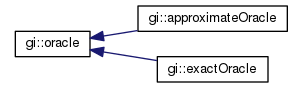
\includegraphics[ width=0.7\textwidth]{EreditaOracolo}
	\caption[Ereditarietà Oracolo]{Ereditarietà Oracolo}
   \label{fig:eor}
\end{figure}

L'algoritmo \ac{ObP} invece di possedere (composizione) un \ac{DFA} target ha un oggetto della classe base astratta Oracolo. Quando invoco il costruttore dell' \ac{ObP}  si deve passare anche l'indirizzo di un oggetto della classe Oracolo. Tramite il tipo di oggetto Oracolo(si ha un handle della classe base Oracolo che punta allo specifico oggetto della classe derivata passato) passato  viene determinato in maniera trasparente con il polimorfismo se si desidera utilizzare l'\ac{ObP} piuttosto che l'\ac{ObPA}. Le chiamate alle funzioni effettuate sull'oggetto Oracolo all'interno di \ac{ObP} hanno la stessa \textit{signature} , cioè le \ac{MQ} e le \ac{EQ} , ma il tipo dell'oggetto Oracolo passato determina automaticamente di quale classe derivata invocare le funzioni (che avranno diverse implementazioni a secondo se appartengono alla classe exactOracle o a quella approximateOracle).  In questo modo la classe dell'algoritmo \ac{ObP} ha subito pochissime modifiche  e il lavoro d'implementazione di questa tesi si è focalizzato sulla classe approximateOracle. Infine all'interno della classe observation\_pack , per impedire al \textit{client} di vedere le strutture dati e le modifiche effettuate su di esse  e in ultimo il modo in cui funziona l'algoritmo, è necessario effettuare una copia interna dell'Oracolo passato dal \textit{client} ma non conoscendo a priori di quale tipo, e quindi di quale classe, è l'Oracolo vi è stata la difficoltà su come invocare il costruttore di copia. A tal fine si è usata la tecnica del \textit{clone idiom} .Quando si ha un riferimento polimorfico cioè un 
  puntatore alla classe base che punta a un oggetto della classe derivata all'occorrenza può sorgere il problema di determinare qual è il tipo della classe derivata . Allora nella classe base si dichiara un metodo virtuale puro che tutte le classi derivate devono quindi implementare. Quest'implementazione consiste nella creazione dinamica  di un nuovo oggetto della classe derivata chiamando il costruttore di copia della classe derivata sull'oggetto corrente (tramite new classeDerivata(*this)). Questo nuovo oggetto creato verrà tornato al chiamante. Si noti che il costruttore di copia della classe derivata deve provvedere a chiamare il costruttore di copia della classe base e che in questi costruttori deve avvenire una deep copy di tutti i membri dinamici.   In figura \ref{fig:cba} l'interfaccia della classe base astratta.
  
 \begin{figure}[htp]
	\centering
	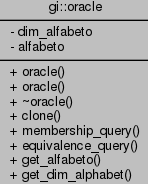
\includegraphics[ width=0.3\textwidth]{Oracolo}
	\caption[Interfaccia classe base Oracolo]{Interfaccia classe base Oracolo}
   \label{fig:cba}
\end{figure}    